\documentclass{article}
%==============================================================================%
%	                          Packages                                     %
%==============================================================================%
% Packages
\usepackage[utf8]{inputenc}
\usepackage{graphicx}
\usepackage{amsmath}
\usepackage{amssymb}
\usepackage{braket}
\usepackage[margin=0.7in]{geometry}
\usepackage[version=4]{mhchem}
\usepackage{float}
%==============================================================================%
%                           User-Defined Commands                              %
%==============================================================================%
% User-Defined Commands
\newcommand{\be}{\begin{equation}}
\newcommand{\ee}{\end{equation}}
\newcommand{\benum}{\begin{enumerate}}
\newcommand{\eenum}{\end{enumerate}}
\newcommand{\pd}{\partial}
\newcommand{\dg}{\dagger}
%==============================================================================%
%                             Title Information                                %
%==============================================================================%
\title{Chem237: Lecture 7}
\date{4/17/18}
\author{Shane Flynn}
%==============================================================================%
\begin{document}
\maketitle

\section*{More Complex Calculus}
Consider
\be
I = \int_0^\infty dx \quad \frac{1}{1+x^3}
\ee
We know that we want to use the residue to compute this integral, so we need to find the poles (which means we need the roots of the associated complex equation). 
\be
\begin{split}
    1 + z^n &= 0 \Rightarrow z^n - 1 = 0\\
    |z|^n = |1|
\end{split}
\ee
So we need exactly n roots (roots of unity), consider the unit circle 

\begin{figure}[H]
  \centering
    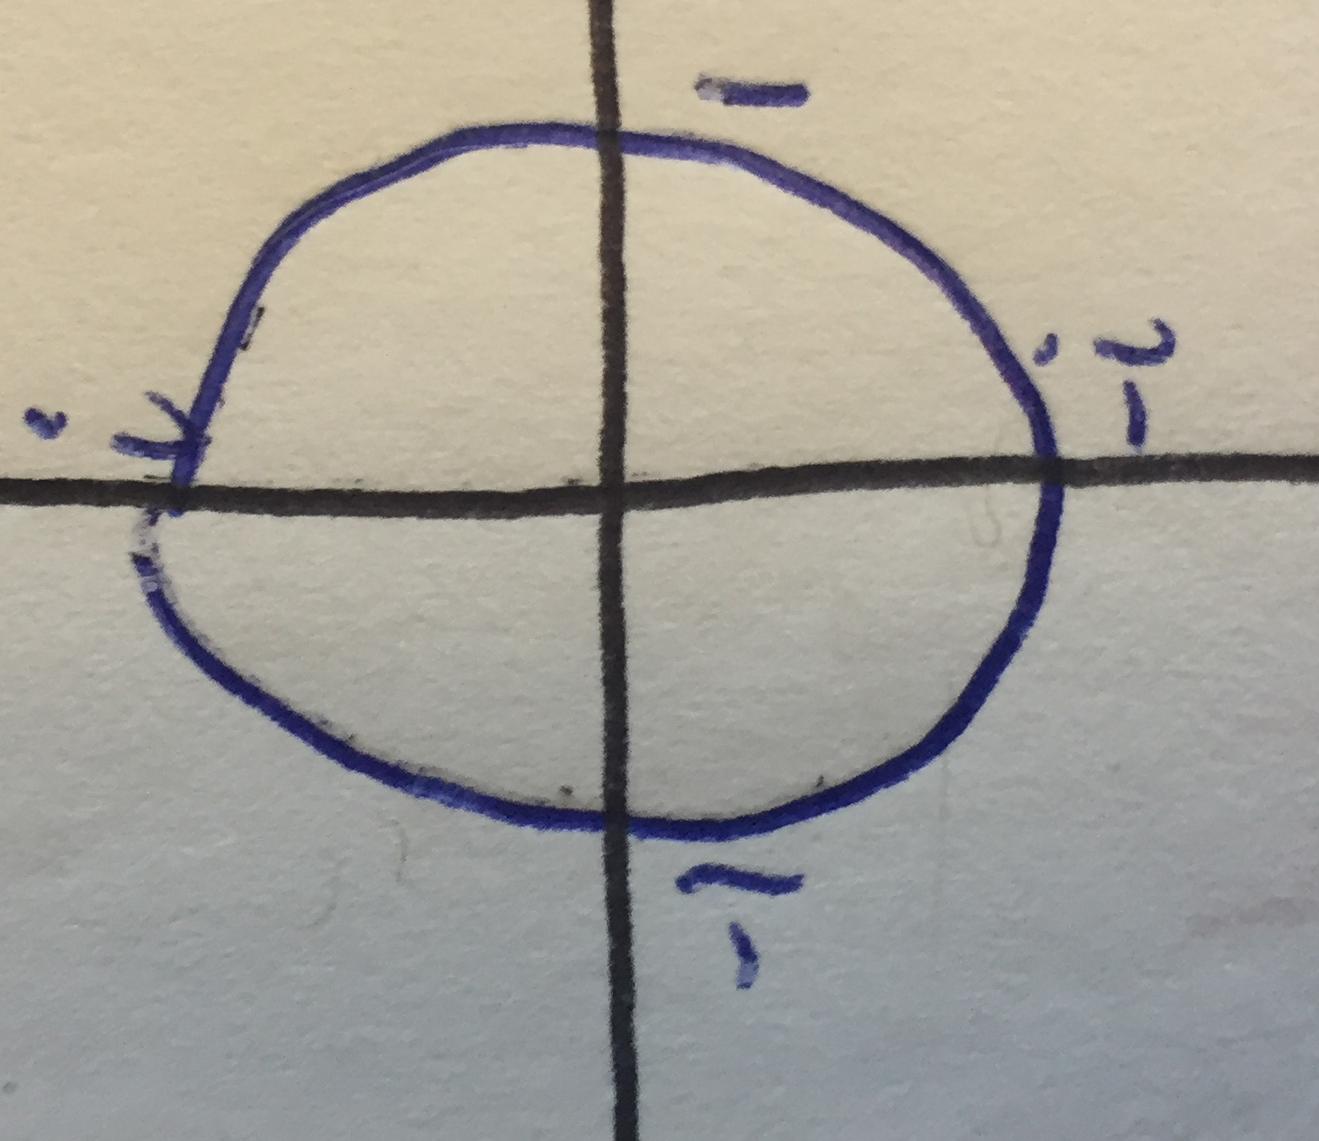
\includegraphics[scale=0.2]{Figures/unit.png}
    \caption{Make a caption. Unit Circle for real/complex}
\end{figure}

All of the roots must be on the unit circle, we can define a complex number z as $z=e^{i\theta}$, which will be on the unit circle. 
\be
1 = e^{ian}, \quad \theta = \frac{2\pi k}{n} \Rightarrow 1 = e^{2\pi ik}
\ee
Where k runs from 0,1,2,3,...,n-1 (to give a total of n roots). 

So we can now find the roots
\be
1+z^n \Rightarrow e^{i\theta n} = 1 - e^{i2\pi k + i\pi} \rightarrow \theta = \frac{2\pi k}{n} + \frac{\pi}{n}
\ee

Returning to our example we can find the first 3 roots for 1 + $|x|^3$ as:  $e^{\frac{i2\pi}{6}}, e^{\frac{-i2\pi}{6}}, -1 $.
So we have foudn our 3 poles for this system. 
\begin{figure}[H]
  \centering
    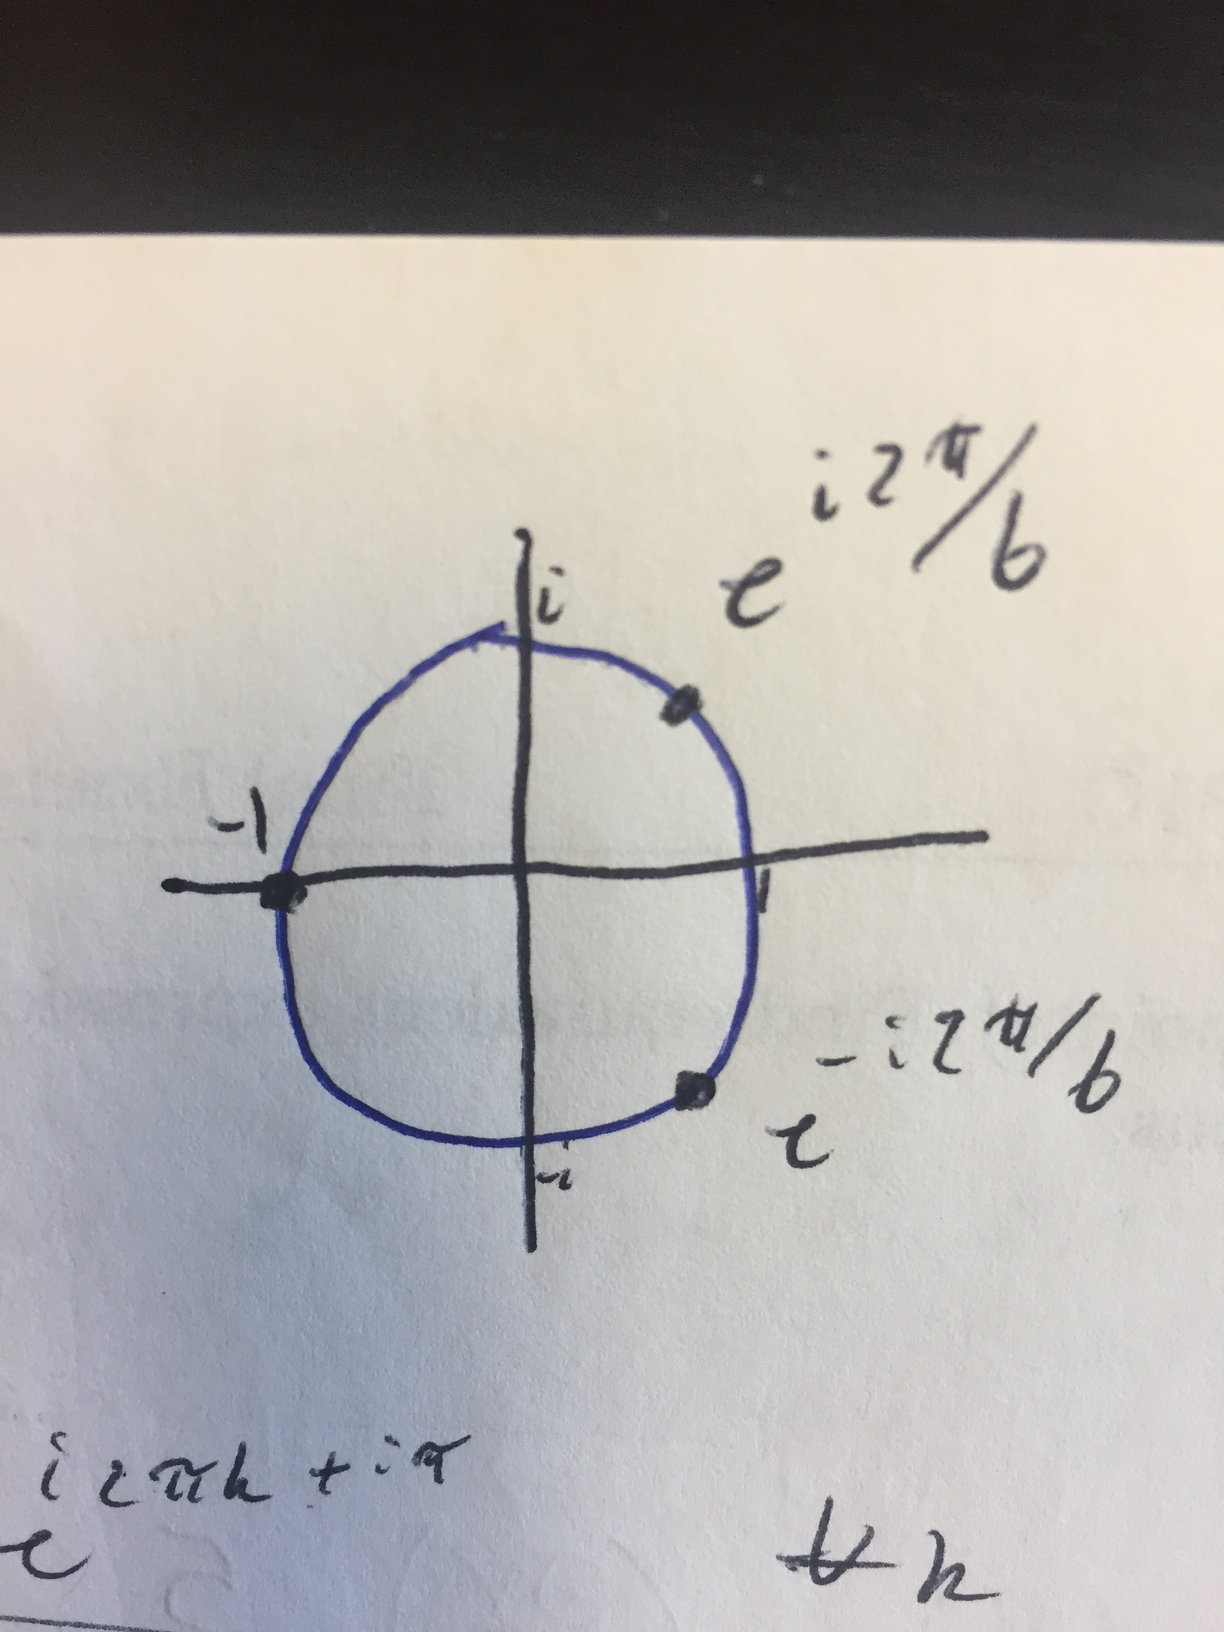
\includegraphics[scale=0.2]{Figures/poles.png}
    \caption{Make a caption. 3 Poles for Cubic Equation}
\end{figure}

But we have a problem now, our integral bounds go from 0 to infinity, our function is not even so we cannot simply change the bounds.

There are two ways we can continue, both will require those poles we just found. 

This first trick is to actually consider a different problem, consider
\be
\oint dz \quad \frac{\ln|z|}{1+z^3}
\ee

Why we are considering this other problem is not clear right now, but we will see.
Unfortunatley the natural logarithm has a branching point, but we can get around this problem (at 0) with an interesting looking contour. 
\begin{figure}[H]
  \centering
    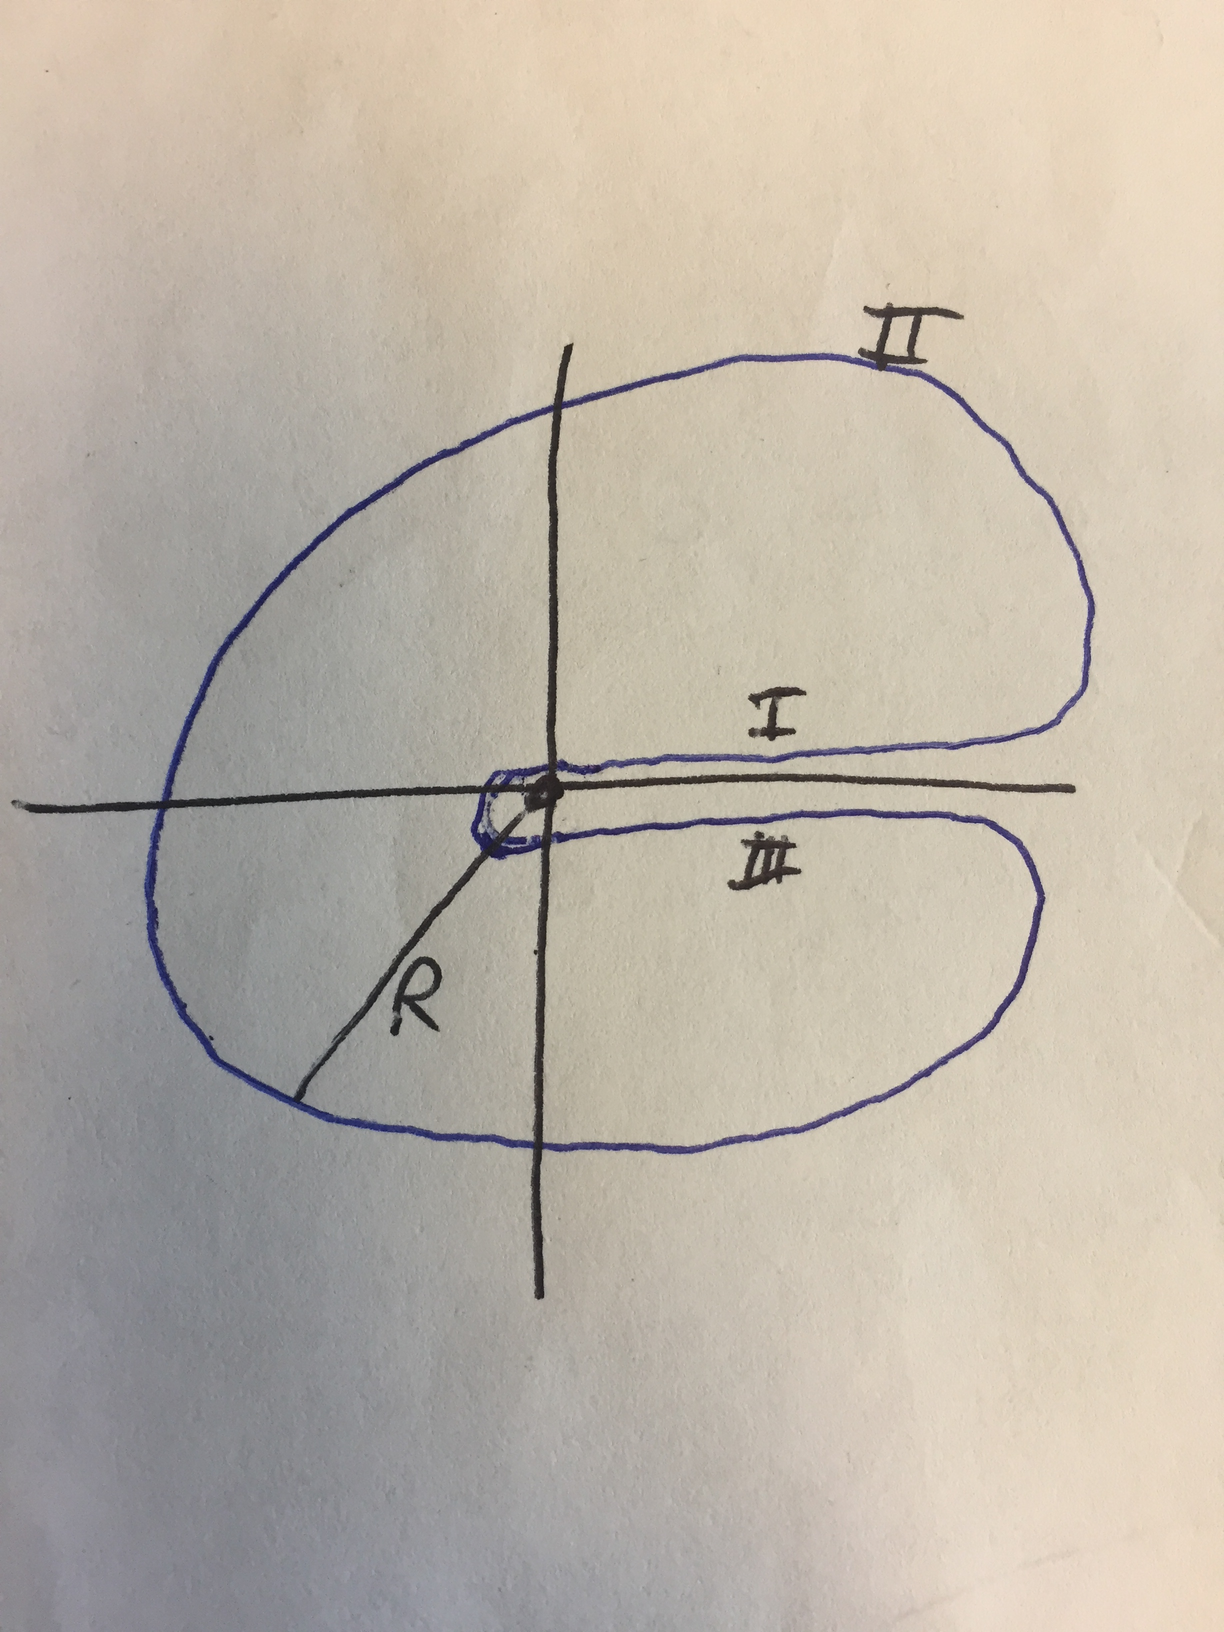
\includegraphics[scale=0.2]{Figures/log.png}
    \caption{Make a caption. I from 0-R, II circle, III R-0. Contour around natural log branching point at 0. ALSO REMEMBER TO PUT THE POLES IN (SAME AS LAST PROBLEM) 3 POLES -1, and the other 2. }
\end{figure}

%%%%%%%%%%%%%%%%%%%%%%%%%%%%%Need to do this math%%%%%%%%%%%%%%%%%%%%%%%%%%%%%%%%%%%%%%%%%%%%%%%%%%%%%%%%%%%%
As usual we start by computing the the limit as R goes to infinity around path II. 
\be
\lim_{R \rightarrow \infty}{\left[\int_0^{2\pi} d\theta \quad Rie^{i\theta} \frac{\ln\left(Re^{i\theta}\right)}{1+R^3e^{3i\theta}}\right]}
\ee
% again let z=re^{i\theta}, dz = Rie^{i\theta}d\theta
This limit again gives 0 so we can evaluate the other pathways to compute our integral of interest. 

With this contour you can do some math and you find the residue to be 
\be
\frac{4\pi^2i\sqrt{3}}{9}
\ee

But we have another problem, our function is not single valued. 
\be
\ln(z) = \lim_{\epsilon\rightarrow 0}{\ln(x+i\epsilon)} = \ln(x)
\ee

Every time we go around the contour (1,0) we pick up a phase factor of ln(x) + 2$\pi$i, therefore
\be
\ln(z) = \ln\left(|z|e^{i2\pi n}\right) = \ln|z| + 2\pi n i
\ee
where n = 0, $\pm$1, $\pm$2 $\cdots$, choosing n=1 we find.
\be
\oint dz \quad \frac{\ln(z)}{1+z^3} = \int_0^R dx \quad \frac{\ln(x)}{1+x^3} + \int_R^0 dx \quad \frac{\ln(x)+2\pi i}{1+x^3} = -2\pi i \int_0^R dx \quad \frac{1}{1+x^3}
\ee
Where we see that our final anser is in terms of the original integral. 
This approach is a general trick for addressing integrals with bounds 0 to infinity. 
%%%%%%%%%%%%%%%%%%%%%%%%%%%%%Need to do this math%%%%%%%%%%%%%%%%%%%%%%%%%%%%%%%%%%%%%%%%%%%%%%%%%%%%%%%%%%%%

A second method for solving this problem is a different contour, again using complex calculus to ocmpute oiur integral of interest. 
\begin{figure}[H]
  \centering
    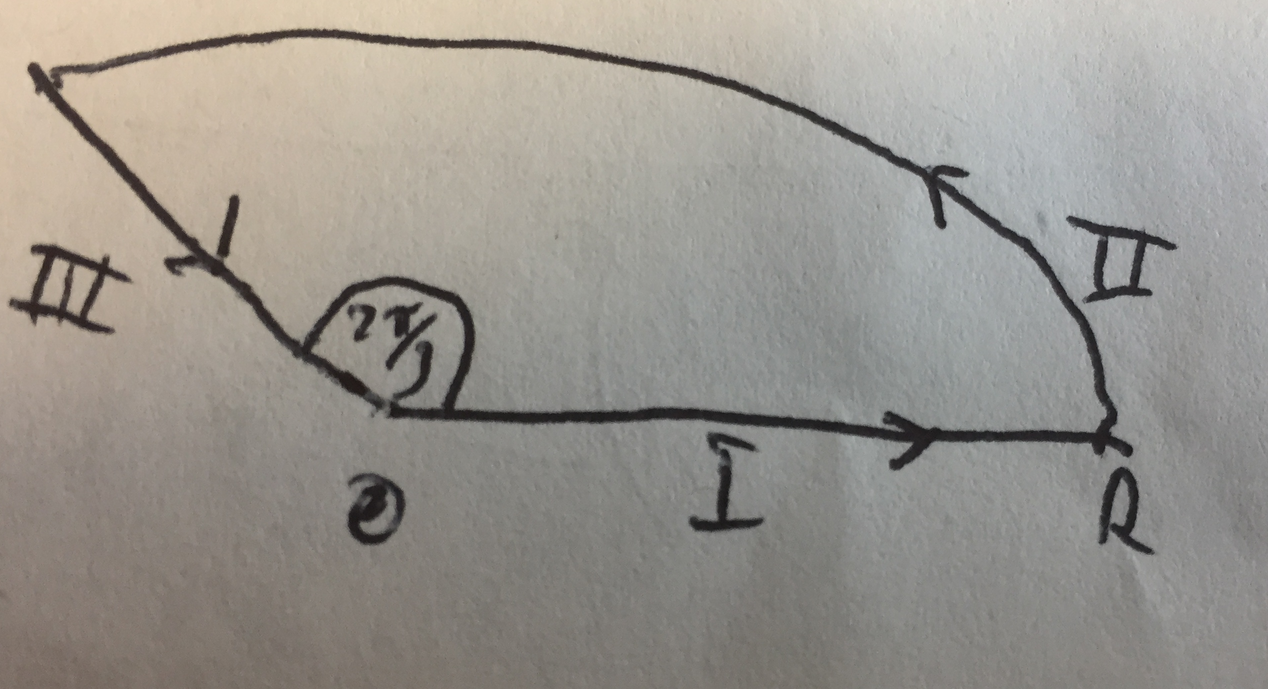
\includegraphics[scale=0.2]{Figures/again.png}
    \caption{Make a caption. Same problem new contour}
\end{figure}
again 3 pathways to compute the closed contour over. 

The first path runs along the integral we are tyring to compute.
\be
I = \int_0^\infty dz \quad \frac{1}{1+x^3}
\ee

Same initial path as before integral II will go to 0.
% dr==> dz 2pii/3.    z=re^{i2[i/3} dz = e^{i2pi/3 dr
\be
III = \int_R^0 dr \quad \frac{e^{2\pi i/3}}{1+r^3} = e^{2\pi i/3} \int_0^R dx \quad \frac{1}{1+x^3}
\ee


\be
\int dz \quad \frac{1}{1+z^3} = I + II + III+ = \left[\int_0^\infty dz \quad \frac{1}{1+x^3}\right] \left(1-e^{2\pi i/3}\right)
\ee

\subsection*{Another Problem}
Assuming A $>$ B $>$ 0
\be
\int_0^\pi d\theta \quad \frac{1}{A+B\cos(\theta)} = \frac{1}{2} \int_0^{2\pi} d\theta \quad \frac{1}{A+B\cos(\theta)}
\ee

We can evaluate this integral using a few substitutions
\be
\begin{split}
    \cos(\theta) &= \frac{e^{i\theta} + e^{-i\theta}}{2} = \frac{z + \frac{1}{z}}{2}\\
    z &= e^{i\theta}, \quad dz = ie^{i\theta} d\theta = izd\theta
\end{split}
\ee

We can now re-write our integral over a closed contour as
\be
\begin{split}
    \oint dz \quad \frac{1}{(iz)A+\frac{B}{2}\left(z+\frac{1}{z}\right)} &= \frac{1}{2} \int_0^{2\pi} d\theta \quad \frac{1}{A+B\cos(\theta)}\\
    & \frac{2}{i} \oint dz \quad \frac{1}{Bz^2 + 2az + B} \rightarrow \text{quadratic}\\
    &= z = \frac{-A}{B} \pm \sqrt{\frac{2a}{B^2}-1} \rightarrow \text{residue theorem}\\
    & \frac{\pi}{\sqrt{A^2 - B^2}}
\end{split}
\ee

So we see another general method, we cna use complex calculus to address trig integrals  over an angle in teh complex unit circle. 

\subsection*{Final Example}
\be
I = \int_0^\infty dz \quad \frac{\sqrt{x}}{1+x^2}
\ee
Because we have the square root there is a branching point at 0, and there are poles at $\pm$ i, so a natural contour for the problem would be the same as used in the natural logarithm problems.

Again with that contour pathway II would go to 0 during the limit and you would need to compute
\be
\int \frac{\sqrt{x}}{1+x^2} - \int \frac{\sqrt{x}}{1+x^2}
\ee
In the limit r to infinity get III = I 


\end{document}
